%% ============================================================
%% 片段：sA-duality   对应原文 PDF 第 146--152 页
%% 本文件由 gw/convert.py 从 arXiv 源码（hep-th/0612073v2）自动生成：
%%   * 公式/编号/引用/图 已经锁定为原文内容，请勿改动任何数学内容与编号；
%%   * 只需把英文正文译为中文，并在每节开头加“本节重点”、关键处加译注。
%% ============================================================


\appendix
%% ==== 原文 Appendix A：PDF 第 146 页（印刷第 145 页）====
\section{对偶性回顾}
\label{sec:A}

\begin{keytakeaways}
  \begin{itemize}[leftmargin=1.4em,itemsep=2pt,topsep=2pt]
    \item \textbf{数学工具}：从根系统的两条公理出发——整性条件~\eqref{eq:A.1} 与关于根的反射封闭性~\eqref{eq:A.2}——构造对偶根系统 $\Phi^\vee$，并建立四组格：根格／权格／特征格与余根格／余权格／余特征格；包含关系~\eqref{eq:A.5}--\eqref{eq:A.7} 在取对偶时全部翻转。
    \item \textbf{关键结论}：朗兰兹（GNO）对偶把 $G$ 与 $^L\neg G$ 的根格与余根格互换，因此二者有相同的外尔群；中心与基本群互换，$\pi_1({}^LG)={\mathcal Z}(G)^\vee$、${\mathcal Z}({}^LG)=\pi_1(G)^\vee$（式~\eqref{eq:A.15}）；单连通型与伴随型互换。
    \item \textbf{关键结论}：非单根系中长短根长度平方之比 $n_{\mathfrak g}$ 等于 $2$（$B,C,F_4$ 型）或 $3$（$G_2$ 型）；取短根长度平方为 $2$ 的度规后，余根由式~\eqref{eq:A.17} 给出，且 $(\mu^*)^*=n_{\mathfrak g}\mu$，$S$-对偶相应写成 $\tau\to-1/n_{\mathfrak g}\tau$。
    \item \textbf{物理图像}：这套根与格的对偶是规范场论中电磁对偶（$S$-对偶）的群论骨架；$B_n$ 与 $C_n$ 互换，而 $F_4$、$G_2$ 作为群自对偶（还需复合一个旋转 $\mathfrak R$），文中图~\ref{fig:8}、图~\ref{fig:9} 给出图示。
  \end{itemize}
\end{keytakeaways}

本附录简要回顾李群（Lie group）$G$ 与其朗兰兹对偶（Langlands dual）或 GNO 对偶群 $^L\neg G$ 之间的关系。一般背景可参看 \cite{ref90} 第 3 章或 \cite{ref91} 第 8 章。为简洁起见，我们只描述 $G$ 单的情形，尽管理论可推广到任意紧李群。

$G$ 的根系统（root system）$\Phi$ 是固定欧氏空间 $\eurme\cong \mathbb{R}^r$ 中的有限个非零向量（$r$ 将是 $G$ 的秩）。$\eurme$ 最终将解释为 $\mathfrak t^\vee$，即 $G$ 的极大环面（maximal torus）$\TT$ 的李代数 $\mathfrak t$ 的对偶。我们认为 $\eurme$ 上赋予了一个度规（metric）$(~,~)$；起初只把它视为在乘以正实标量意义下确定的量，稍后我们将选定一个特定的度规。

要求 $\Phi$ 满足若干公理。$\Phi$ 中的向量生成一个秩为 $r$ 的格 $\Lambda_\rt$（最终解释为 $G$ 的根格（root lattice）），它不能分解为若干相互正交的子格之直和。此外，
%\footnote{We follow \cite{ref90}\ and
%much of the literature in writing $\alpha,\beta$
%for roots of a Lie algebra,
%hoping that this will cause no serious
%confusion with the use of $\alpha,\beta,\gamma$
%in the body of this paper to denote parameters of
%a surface operator.}
对 $\mu\in \Phi$，要求 $\Phi$ 中所含 $\mu$ 的倍数恰为向量 $\pm \mu$。这将保证 $\mathfrak{g}$ 中存在以 $\pm \mu$ 为非零根（root）的 $\mathfrak{sl}(2)$ 子代数；我们称此代数为 $\mathfrak{sl}(2)_\mu$。我们还要求：对任意其它根 $\nu$，表达式
% 式 (A.1)
\setcounter{equation}{0}
\begin{equation}\label{eq:A.1}
  \langle\nu,\mu\rangle ={2(\nu,\mu)\over (\mu,\mu)}
\end{equation}
为整数。注意符号 $\langle~,~\rangle$ 与 $(~,~)$ 的归一化无关，且只对第一个变量线性。$\langle\nu,\mu\rangle$ 的整性可解释为：每个根 $\nu$ 关于 $\mathfrak{sl}(2)_\mu$ 具有整数或半整数权（weight）。最后，要求根集在关于 $\mu$ 的反射（reflection）下封闭，该反射即运算
% 式 (A.2)
\setcounter{equation}{1}
\begin{equation}\label{eq:A.2}
  \nu\to \nu-\langle\nu,\mu\rangle \mu.
\end{equation}

此运算最终被解释为代数 $\mathfrak{sl}(2)_\mu$ 的外尔变换（Weyl transformation）。

对任何这样的根系统 $\Phi$，可按如下方式定义对偶根系统（dual root system）$\Phi^\vee$。对 $\mu\in \Phi$，定义
% 式 (A.3)
\setcounter{equation}{2}
\begin{equation}\label{eq:A.3}
  \mu^\vee={2\mu\over (\mu,\mu)}.
\end{equation}

$\Phi^\vee$ 恰由对应于 $\mu\in\Phi$ 的向量 $\mu^\vee$ 构成。一个简短的计算表明 $\Phi^\vee$ 满足与 $\Phi$ 相同的公理。它将解释为对偶群的根系统。

\begin{yizhu}[含糊点拨]
作者的“简短计算”实际要验证三件事，其中只有后两件需要一点计算：(i) $\mu^\vee$ 是 $\mu$ 的正倍数，故“$\Phi$ 中 $\mu$ 的倍数只有 $\pm\mu$”在 $\Phi^\vee$ 中自动成立；(ii) 整性：$\langle\nu^\vee,\mu^\vee\rangle=\dfrac{2(\nu^\vee,\mu^\vee)}{(\mu^\vee,\mu^\vee)}=\dfrac{2(\nu,\mu)}{(\nu,\nu)}=\langle\mu,\nu\rangle\in\Z$（用到 $(\nu^\vee,\mu^\vee)=4(\nu,\mu)/((\nu,\nu)(\mu,\mu))$）；(iii) 反射封闭：$\nu^\vee-\langle\nu^\vee,\mu^\vee\rangle\mu^\vee$ 恰是 $(\nu-\langle\nu,\mu\rangle\mu)^\vee$，同样代入上式即得。注意整性中出现的次序是 $\langle\mu,\nu\rangle$ 而非 $\langle\nu,\mu\rangle$：检验 $\Phi^\vee$ 的公理时以 $\mu^\vee$ 为“根”，于是 $\mu$ 与 $\nu$ 的角色互换。
\end{yizhu}

然而，$\mu^\vee$ 的定义依赖于度规 $(~,~)$ 的归一化，因此向量 $\mu^\vee$ 其实并不自然地是 $\eurme$ 中的向量；更自然的是把它们理解为对偶空间（dual space）$\eurme^\vee$ 中的向量。理由如下：对 $\mu,\nu\in \Phi$，配对（pairing）
% 式 (A.4)
\setcounter{equation}{3}
\begin{equation}\label{eq:A.4}
  \mu^\vee(\nu)=(\nu,\mu^\vee)={2(\nu,\mu)\over (\mu,\mu)}=
\langle \nu,\mu\rangle
\end{equation}
与度规 $(~,~)$ 的归一化无关。因此，原根系统 $\Phi$ 位于 $\eurme\cong \mathfrak t^\vee$ 中，而对偶根系统 $\Phi^\vee$ 位于 $\eurme^\vee\cong \mathfrak t$ 中。

$\Phi$ 的外尔群（Weyl group）$\mathcal W$ 是由关于诸根 $\mu$ 的反射生成的群，即运算 $\nu\to\nu-\mu\langle\nu,\mu\rangle$。类似地，$\Phi^\vee$ 的外尔群 $\mathcal W^\vee$ 由关于诸余根（coroot）$\mu^\vee$ 的反射生成，即 $\nu\to\nu-\mu^\vee\langle\nu,\mu^\vee\rangle$。但由于 $\mu^\vee$ 是 $\mu$ 的实倍数，有 $\mu\langle\nu,\mu\rangle=\mu^\vee\langle\nu,\mu^\vee\rangle$，故关于 $\mu$ 与关于 $\mu^\vee$ 的反射相同。因此群 $\mathcal W$ 与 $\mathcal W^\vee$ 也相同。这导致 $G$ 与其对偶群 $^L\neg G$ 有相同的外尔群。

正如向量 $\mu\in\Phi$ 生成秩 $r$ 的格 $\Lambda_\rt$，向量 $\mu^\vee\in\Phi^\vee$ 生成秩 $r$ 的格 $\Lambda_\cort$（余根格（coroot lattice））。我们用 $\Lambda_\cowt$（余权格（coweight lattice））表示 $\Lambda_\rt$ 的对偶格，用 $\Lambda_\wt$（权格（weight lattice））表示 $\Lambda_\cort$ 的对偶格。于是（暂时借助度规 $(~,~)$ 把这些格都看作嵌入在 $\eurme$ 中），$\nu\in\Lambda_\cowt$ 当且仅当对一切 $\mu\in\Phi$ 有 $(\nu,\mu)\in\Z$；$\nu\in\Lambda_\wt$ 当且仅当对一切 $\mu^\vee\in\Phi^\vee$ 有 $(\nu,\mu^\vee)\in\Z$。对 $\nu\in \Lambda_\rt$、$\mu^\vee\in\Lambda_\cort$，配对 $(\nu,\mu^\vee)$ 的整性意味着有如下包含关系
% 式 (A.5)
\setcounter{equation}{4}
\begin{equation}\label{eq:A.5}
  \begin{aligned}\Lambda_\rt & \subset \Lambda_\wt \\
                    \Lambda_\cort & \subset\Lambda_\cowt.\end{aligned}
\end{equation}

这些格都有相同的秩 $r$，故这些包含关系的指数有限。

现在令 $\Lambda_\char$（特征格（character lattice））为介于 $\Lambda_\rt$ 与 $\Lambda_\wt$ 之间的任意格：
% 式 (A.6)
\setcounter{equation}{5}
\begin{equation}\label{eq:A.6}
  \Lambda_\rt\subset \Lambda_\char\subset\Lambda_\wt.
\end{equation}

$\Lambda_\char$ 的对偶是格 $\Lambda_\cochar$（余特征格（cocharacter lattice）），它介于余根格与余权格之间：
% 式 (A.7)
\setcounter{equation}{6}
\begin{equation}\label{eq:A.7}
  \Lambda_\cort\subset \Lambda_\cochar\subset\Lambda_\cowt.
\end{equation}

当然，式~\eqref{eq:A.7} 中的三个格自然地看作嵌入在 $\eurme^\vee$ 中；它们在 $\eurme$ 中的嵌入依赖于度规 $(~,~)$ 的选取。

紧单李群的分类表明，这类群对应于在此类构造中能出现的特征格。对每个 $\Lambda_\char$ 的选取，都存在一个紧李群 $G$，使得 $G$ 的某个表示的最高权是 $\Lambda_\char$ 中的元素。事实上，$\Lambda_\char$ 就是特征群，即 $G$ 的极大环面 $\mathbb{T}$ 到 $U(1)$ 的同态构成的群。因此
% 式 (A.8)
\setcounter{equation}{7}
\begin{equation}\label{eq:A.8}
  \Lambda_\char={\rm Hom}(\mathbb{T},U(1)),
\end{equation}
对偶地，
% 式 (A.9)
\setcounter{equation}{8}
\begin{equation}\label{eq:A.9}
  \Lambda_\cochar={\rm Hom}({}^L\neg\TT,U(1))={\rm Hom}(U(1),\mathbb{T}).
\end{equation}

若 $\Lambda_\char=\Lambda_\wt$，则 $G$ 单连通（simply-connected）；若 $\Lambda_\char=\Lambda_\rt$，则 $G$ 为伴随型（adjoint type）。

更一般地，记 ${\mathcal Z}(G)$ 为 $G$ 的中心（center）。对任意局部紧阿贝尔群（locally compact abelian group）$A$，记 $A^\vee$ 为 ${\rm Hom}(A,U(1))$；按庞特里亚金对偶（Pontryagin duality），若 $B=A^\vee$，则 $A=B^\vee$。在 $G$ 的不可约表示（irreducible representation）$R$ 中，${\mathcal Z}(G)$ 中心地作用，换言之通过一个到 $U(1)$ 的同态作用。$R$ 的最高权是元素 $w\in\Lambda_\char$；当 $w\in\Lambda_\rt$ 时 ${\mathcal Z}(G)$ 平凡地作用。商 $\Lambda_\char/\Lambda_\rt$ 就是 ${\rm Hom}({\mathcal Z}(G),U(1))$：
% 式 (A.10)
\setcounter{equation}{9}
\begin{equation}\label{eq:A.10}
  {\mathcal Z}(G)^\vee = \Lambda_\char/\Lambda_\rt.
\end{equation}

利用式~\eqref{eq:A.6} 与式~\eqref{eq:A.7} 中诸包含关系之间的对偶性，这等价于
% 式 (A.11)
\setcounter{equation}{10}
\begin{equation}\label{eq:A.11}
  {\mathcal Z}(G)=\Lambda_\cowt/\Lambda_\cochar.
\end{equation}

类似地，基本群（fundamental group）$\pi_1(G)$ 中的一个元素，若提升到 $G$ 的泛覆盖（universal cover）$\bar G$，就确定了一条从单位元到 $\bar G$ 的某中心元 $\xi$ 的路径。在 $\bar G$ 的表示 $R$ 中，$\xi$ 通过乘以 $U(1)$ 中某个元素而作用。按此构造，$R$ 确定了 $\pi_1(G)^\vee$ 中的一个元素；若 $R$ 实际上是 $G$ 的表示（即其最高权在 $\Lambda_\char$ 中），则该元素为零。由此得到关系
% 式 (A.12)
\setcounter{equation}{11}
\begin{equation}\label{eq:A.12}
  \pi_1(G)^\vee=\Lambda_\wt/\Lambda_\char.
\end{equation}

同样，式~\eqref{eq:A.6} 与式~\eqref{eq:A.7} 之间的对偶性给出另一版本
% 式 (A.13)
\setcounter{equation}{12}
\begin{equation}\label{eq:A.13}
  \pi_1(G)=\Lambda_\cochar/\Lambda_\cort.
\end{equation}

朗兰兹对偶或 GNO 对偶群 $^L\neg G$ 与格 $\Lambda_\cort,$ $\Lambda_\cochar$、$\Lambda_\cowt$ 的关系，恰如 $G$ 与 $\Lambda_\rt$、$\Lambda_\char$、$\Lambda_\wt$ 的关系。以上所有陈述都有显然的对偶。例如，若 $\Lambda_\cochar=\Lambda_\cowt$，则 $^L\neg G$ 单连通；若 $\Lambda_\cochar=\Lambda_\cort$，则它为伴随型。更一般地，
% 式 (A.14)
\setcounter{equation}{13}
\begin{equation}\label{eq:A.14}
  \begin{aligned}
{\mathcal Z}({}^L\neg G)^\vee&=\Lambda_\cochar/\Lambda_\cort\\
\pi_1({}^L\neg G)^\vee& = \Lambda_\cowt/\Lambda_\cochar.\end{aligned}
\end{equation}

把式~\eqref{eq:A.14} 与式~\eqref{eq:A.11}、式~\eqref{eq:A.13} 相比较，可知
% 式 (A.15)
\setcounter{equation}{14}
\begin{equation}\label{eq:A.15}
  \begin{aligned}\pi_1({}^LG)&={\mathcal Z}(G)^\vee\\
                     {\mathcal Z}({}^LG)&=\pi_1(G)^\vee.\end{aligned}
\end{equation}

整个构造在以下交换下完全对称：把 $\eurme$ 与 $\eurme^\vee$ 互换，把式~\eqref{eq:A.6} 中的格与式~\eqref{eq:A.7} 中的对偶格互换，并把群 $G$ 与对偶群 $^L\neg G$ 互换。在李代数理论中，$G$ 的根取值于 $\mathfrak t^\vee$（极大环面的李代数 $\mathfrak t$ 的对偶），而余根取值于 $\mathfrak t$，故我们把 $\eurme$ 等同于 $\mathfrak t^\vee$、把 $\eurme^\vee$ 等同于 $\mathfrak t$。式~\eqref{eq:A.11} 与式~\eqref{eq:A.13} 的结果有更直接的解释：格 $\Lambda_\cort,$ $\Lambda_\cochar$、$\Lambda_\cowt$ 都自然地嵌入 $\mathfrak t$。

\bigskip\noindent{\it 度规的选择}

此时，对 $\eurme$ 上的度规 $(~,~)$ 作一个方便的选取是有益的。

若 $\Phi$ 中所有根 $\mu$ 的长度平方相同，则称群 $G$ 为单根系（simply-laced）。这恰在 $G$ 为 $ {A}$、$ {D}$、$ {E}$ 型时发生。此时方便地选取使诸根长度平方恰为 $2$ 的度规，即对一切 $\mu$ 有 $(\mu,\mu)=2$。回顾式~\eqref{eq:A.3} 中 $\mu^\vee$ 的定义可见，此条件保证对一切 $\mu$ 有 $\mu^\vee=\mu$。这使上面概述的构造简化：$\eurme$ 与 $\eurme^\vee$ 的区别可以略去而不损失任何对称性，于是 $\Lambda_\rt=\Lambda_\cort$、$\Lambda_\wt=\Lambda_\cowt$。在此情形，群 $G$ 与 $^L\neg G$ 有相同的李代数（因为它们的根格相同），但未必同构（因为格 $\Lambda_\char$ 与 $\Lambda_\cochar$ 可以不同）。

现在考虑 $G$ 非单根系的情形。此时，由单李代数的分类可知，根的长度平方恰有两个取值。我们把这二者之比记为 $n_{\mathfrak g}$；对 $ {B}$、$ {C}$ 或 $ {F}_4$ 型群它等于 $2$，对 $ {G}_2$ 等于 $3$。由 $\mu^\vee=2\mu/(\mu,\mu)$ 得
% 式 (A.16)
\setcounter{equation}{15}
\begin{equation}\label{eq:A.16}
  (\mu^\vee,\mu^\vee)={4\over (\mu,\mu)}.
\end{equation}

因此函数 $(\mu^\vee,\mu^\vee)$ 对 $\mu^\vee\in\Phi^\vee$ 仍取两个值，且这两个值之比同样是 $n_{\mathfrak g}$。此外，由式~\eqref{eq:A.16} 可见：若 $\mu$ 是短根，则 $\mu^\vee$ 是长余根；若 $\mu$ 是长根，则 $\mu^\vee$ 是短余根。

\begin{yizhu}[易错点]
本节最易出错之处是长度平方的归一化。$n_{\mathfrak g}$ 是同一条根系统中长根与短根长度平方之比，只能取 $2$（$B,C,F_4$ 型）或 $3$（$G_2$ 型）；对单根系无长短之分，即 $n_{\mathfrak g}=1$。文献中有两种常用约定：(i) 长根长度平方取 $2$；(ii) 短根长度平方取 $2$（本文及本文的规范场论部分所用，它使式~\eqref{eq:A.17} 中短根情形最简单：$\mu^\vee=\mu$）。两种约定的度规相差因子 $n_{\mathfrak g}$（等价地，长度相差 $\sqrt{n_{\mathfrak g}}$），故引用公式前必须先确认采用哪一种，否则 $n_{\mathfrak g}$ 的位置以及 $1/\sqrt3$、$1/\sqrt2$ 等因子都会对不上。注意 $\mu^\vee=2\mu/(\mu,\mu)$ 依赖度规归一化，而不依赖归一化的是配对数 $\langle\nu,\mu\rangle$（式~\eqref{eq:A.4}）。
\end{yizhu}

% [FIGURE 8] 原文 PDF 第 150 页；caption 见下，需翻译
\begin{figure}[htbp]
  \centering
  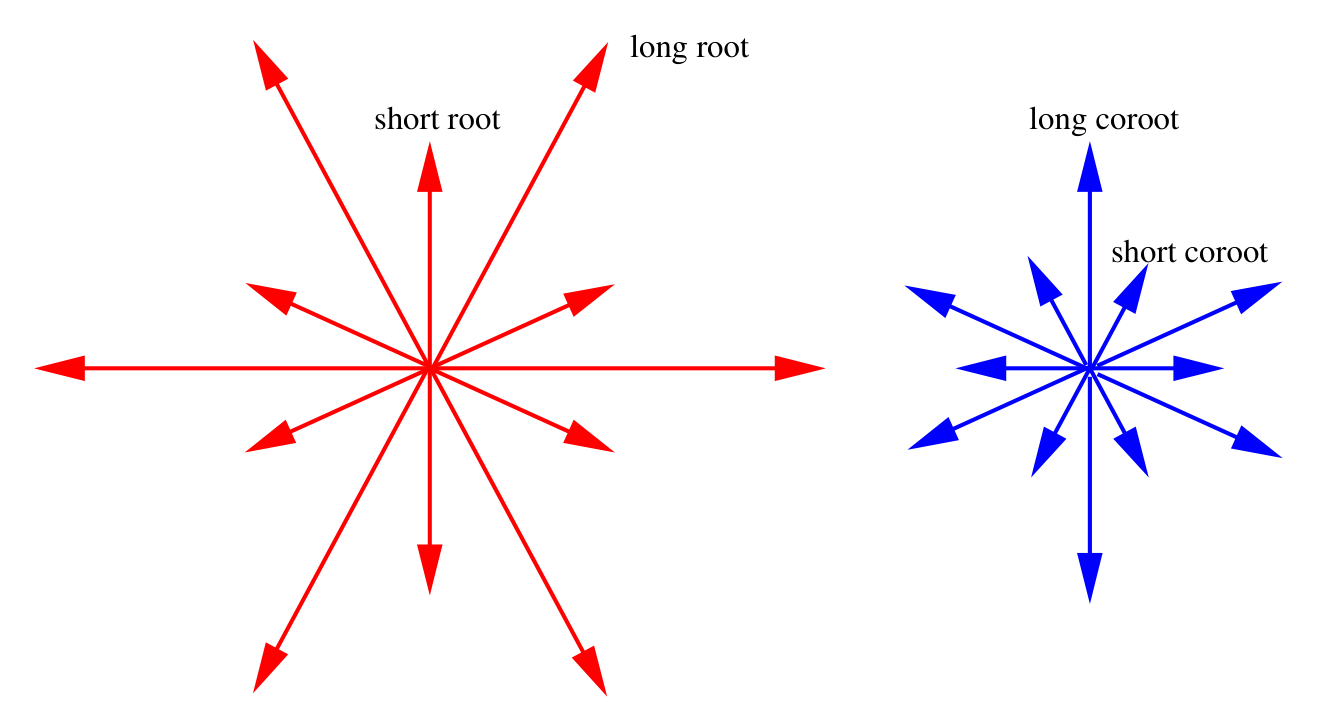
\includegraphics[width=0.62\linewidth]{figures/figure-8.png}
  \caption{此处展示李群 $ {G}_2$ 的根（左）与余根（右）。映射 $\mu\to\mu^*$（用短根长度平方为 $2$ 的度规定义）把左侧的向量映到右侧的“同一个”向量：短根映为长余根，长根映为短余根的 $3$ 倍。要得到根图与余根图之间的同构，可以把映射 $\mu\to\mu^*$ 与角度为 $\pm \pi/6$ 的旋转以及乘以 $1/\sqrt 3$ 复合。（原文 Fig.~8，PDF 第 150 页）}
  \label{fig:8}
\end{figure}

此时我们显然不能把 $\eurme$ 上的度规 $(~,~)$ 归一化得让所有根的长度平方都为 $2$。不过，方便的是把度规归一化得让短根的长度平方为 $2$，于是长根的长度平方为 $2n_{\mathfrak g}$。作此选择后，有
% 式 (A.17)
\setcounter{equation}{16}
\begin{equation}\label{eq:A.17}
  \mu^\vee = \begin{cases} \mu & \text{若 $\mu$ 是短根；}\\ {\mu/ n_{\mathfrak g}} & \text{若 $\mu$ 是长根。}\end{cases}
\end{equation}

反过来，有
% 式 (A.18)
\setcounter{equation}{17}
\begin{equation}\label{eq:A.18}
  \mu = \begin{cases} \mu^\vee & \text{若 $\mu$ 是短根；}\\ n_{\mathfrak g}{\mu^\vee} & \text{若 $\mu$ 是长根。}\end{cases}
\end{equation}

一旦选定度规，我们就得到 $\eurme$ 与 $\eurme^\vee$ 的自然等同。这给出从 $\eurme$ 到 $\eurme^\vee$ 的映射，把 $\nu\in\eurme$ 映为由 $\nu(\mu)=(\nu,\mu)$ 定义的 $\eurme$ 上的线性形式。我们记此映射为 $\nu\to\nu^*$。由式~\eqref{eq:A.18} 可以更精确：若 $\mu\in\Phi$ 是短根，则 $\mu^*$（它与 $\mu$ 相同，只是解释为 $\eurme^\vee$ 中的元素）等于长余根（即 $\mu^\vee$）；但若 $\mu$ 是长根，则 $\mu^*$ 是短余根 $\mu^\vee$ 的 $n_{\mathfrak g}$ 倍。对 $ {G}_2$ 的情形，图~\ref{fig:8} 说明了这一点。特别地，$\mu^*$ 不总是余根，但总在余根格中，故线性变换 $\mu\to\mu^*$ 把 $\Lambda_\rt$ 映入 $\Lambda_\cort$。

当然，此构造也有对偶版本。我们可以在 $\eurme^\vee$ 上选取使短余根长度平方为 $2$ 的度规。这给出自然的映射 $\eurme^\vee\to \eurme$，记作 $\mu^\vee\to (\mu^\vee)^*$。用同样的推理可知，此运算把短余根映为长根，把长余根映为短根的 $n_{\mathfrak g}$ 倍。特别地，它把 $\Lambda_\cort$ 映入 $\Lambda_\rt$。

两个映射的复合是乘以 $n_{\mathfrak g}$，即对一切 $\mu$ 有 $(\mu^*)^*=n_{\mathfrak g}\mu$。事实上，短根先映为长余根，再映为原短根的 $n_{\mathfrak g}$ 倍；而长根先映为短根的 $n_{\mathfrak g}$ 倍，再映为原长根的 $n_{\mathfrak g}$ 倍。

\begin{yizhu}[易错点]
$\mu\to\mu^*$ 与旋转 $\mathfrak R$ 的次序不可随意交换。$\mu\to\mu^*$ 是（选定度规后）$\eurme\to\eurme^\vee$ 的线性映射；而 $\mathfrak R:\eurme^\vee\to\eurme$ 是反方向的映射（作者对此有明言），它先用 $\eurme^\vee$ 上“短余根长度平方为 $2$”的度规把 $\eurme^\vee$ 与 $\eurme$ 等同，再作旋转。因此从根图到余根图的同构是 $\mathfrak R\circ(\mu\to\mu^*)$（先取星号，再旋转）：$\mu^*$ 已把长根压成 $n_{\mathfrak g}$ 倍的短余根，$\mathfrak R$ 中的因子 $1/\sqrt{n_{\mathfrak g}}$（$G_2$ 为 $1/\sqrt3$，$F_4$ 为 $1/\sqrt2$）正是把长度重新标回原根长度所必需的；$\mathfrak R$ 的旋转部分负责把方向转对，使长根方向落到原短根方向。模去外尔变换后，$\mathfrak R$ 由“交换邓金图两端”唯一确定。若颠倒次序（先旋转再取星号），一般只差一个外尔变换，但标度因子会错位。
\end{yizhu}

\bigskip\noindent{\it 邓金图}

若 $r$ 个根 $\mu_i\in\Phi$ 使得每个根 $\mu$ 都有展开 $\mu=\sum_i a_i\mu_i$，其中系数 $a_i$ 全非负或全非正，则称这组根为一组单正根（simple positive roots）。这样的集合总存在，且在相差一个外尔变换的意义下唯一。

若 $\mu_i$ 是 $\Phi$ 的一组单正根，则对偶根 $\mu_i^\vee\in\Phi^\vee$ 是 $\Phi^\vee$ 的一组单正根。事实上，各 $\mu_i^\vee$ 是 $\mu_i$ 的正倍数，而任意对偶根 $\mu^\vee$ 与 $\mu$ 也有同样的关系。因此在展开 $\mu^\vee=\sum_ib_i \mu_i^\vee$ 中，系数 $b_i$ 与 $\mu=\sum_ia_i\mu_i$ 中的系数 $a_i$ 同号。

$G$ 的邓金图（Dynkin diagram）对每个单正根有一个节点（node）；节点的连接方式编码了单正根之间的夹角。当 $G$ 非单根系时，图中通常还标有一个从长根指向短根的箭头（arrow）。

% [FIGURE 9] 原文 PDF 第 151 页；caption 见下，需翻译
\begin{figure}[htbp]
  \centering
  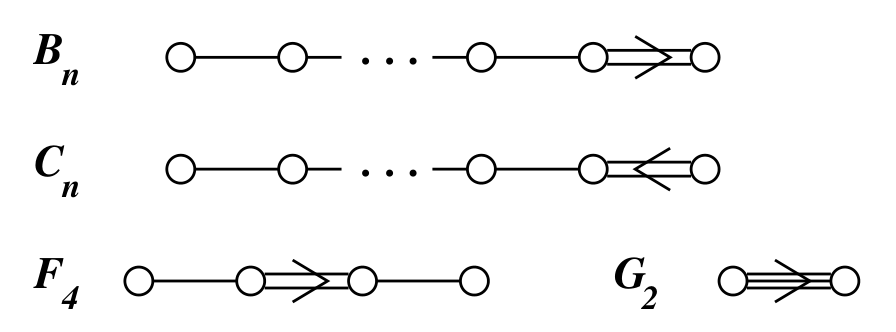
\includegraphics[width=0.62\linewidth]{figures/figure-9.png}
  \caption{非单根系李群的邓金图。对偶的作用是把从长根指向短根的箭头反向。因此群 $B_n$ 与 $C_n$ 在对偶下互换。然而，$F_4$ 与 $G_2$ 是自对偶的，因为对这两个群而言，箭头反向等价于交换图的两端。（原文 Fig.~9，PDF 第 151 页）}
  \label{fig:9}
\end{figure}

$\Phi$ 的单正根 $\mu_i$ 之间的夹角与 $\Phi^\vee$ 的单正根 $\mu_i^\vee$ 之间的夹角相同，因为 $\mu_i^\vee$ 是 $\mu_i$ 的正倍数。然而，如上面所见，变换 $\mu\to\mu^\vee$ 把短根映为长根、把长根映为短根。因此根系统 $\Phi$ 与 $\Phi^\vee$ 的邓金图看起来完全相同，只是在非单根系情形箭头的方向相反。图~\ref{fig:9} 说明了这一点。

\begin{yizhu}[易错点]
读图~\ref{fig:9} 时注意三点：(i) 文中箭头约定为“从长根指向短根”，有些文献相反；若约定相反，$B_n$ 与 $C_n$ 的图形会对调，容易误判哪一对在对偶下互换。(ii) 对偶把 $\Phi$ 换成 $\Phi^\vee$ 的效果是箭头反向，故 $B_n$ 与 $C_n$ 互换；而 $F_4$、$G_2$ 的邓金图在箭头反向后与自身重合（对 $F_4$ 须同时交换两端的节点，对 $G_2$ 即交换三重节点与单重节点）。(iii) 图的重合只给出李代数的同构；要得到群层面的自对偶，还须把 $\mu\to\mu^*$ 与 $\mathfrak R$ 复合（见上文），使根格与余根格相配，而 $\mu\to\mu^*$ 本身并不是 $\Phi$ 与 $\Phi^\vee$ 的同构。
\end{yizhu}

$G$ 的列维子群（Levi subgroup）$\mathbb{L}$ 的邓金图由 $G$ 的邓金图去掉若干节点得到。$^L\neg G$ 有相应的列维子群 $^L\mathbb{L}$，其邓金图由“同样的”节点组成。$\mathbb{L}$ 与 $^L\mathbb{L}$ 有相同的外尔群，理由与 $G$ 和 $^L\neg G$ 相同。

\bigskip\noindent{\it 与规范场论的比较}

对单根系 $G$，使根长度平方为 $2$ 的度规在对偶下不变，因为在此度规下根与余根重合。

当 $G$ 非单根系时，若用使根长度平方为 $2$ 或 $2n_{\mathfrak g}$ 的度规把 $\eurme$ 与其对偶等同，则余根的长度平方为 $2$ 或 $2/n_{\mathfrak g}$，故此方案在对偶下并不不变。公式 $(\mu^*)^*=n_{\mathfrak g}\mu$ 中的因子 $n_{\mathfrak g}$ 反映了这一不对称，$S$-对偶变换 $\tau\to -1/n_{\mathfrak g}\tau$ 中的因子 $n_{\mathfrak g}$ 同样如此。

当然，只要把度规除以 $\sqrt{n_{\mathfrak g}}$ 就能恢复对偶性。然而，这会使其它公式变得别扭。事实上，使短余根长度平方为 $2$ 的 $\mathfrak t\cong \eurme^\vee$ 上的度规在规范场论中被广泛使用，例如本文从第~\ref{sec:2.4}~节与第~\ref{sec:2.5}~节起就采用它，因为它给出的瞬子数（instanton number）\eqref{eq:2.39} 与 $\theta$ 角（theta-angle）\eqref{eq:2.38} 的定义对所有 $G$ 一致有效。

此外，按我们所作的方式归一化度规还有一优点：由此得到的映射 $\mu\to\mu^*$ 与 $\mu^\vee\to (\mu^\vee)^*$ 虽不是相应格的同构，却把 $\Lambda_\rt$ 映入 $\Lambda_\cort$、反之亦然。若除以 $\sqrt{n_{\mathfrak g}}$，这一性质就失去了。

\begin{yizhu}[物理图像补充]
这一节解释了本文自始至终采用“短余根长度平方为 $2$”的度规（自第~\ref{sec:2.4}~节与第~\ref{sec:2.5}~节起）的原因：规范场论中 $\tau=\theta/2\pi+4\pi i/g^2$ 的虚部与瞬子数、$\theta$ 角的定义都按此归一化，从而式~\eqref{eq:2.38}、\eqref{eq:2.39} 对所有 $G$ 统一。代价是 $S$-对偶不能写成简单的 $\tau\to-1/\tau$，而须写成 $\tau\to-1/n_{\mathfrak g}\tau$：非单根系中长根与短根的李代数数据相差因子 $n_{\mathfrak g}$，$S$-对偶在交换电磁荷的同时也要把二者互换。物理上，$n_{\mathfrak g}$ 的出现正反映了非单根系规范场论中 Wilson 与 't Hooft 算符的对偶交换；若采用把 $\mathfrak R$ 并入 $S$ 的约定 \cite{ref41,ref42}，可把 $G_2$、$F_4$ 的自对偶写得显然，但那要牺牲公式对所有群的一致性，本文选择后者。
\end{yizhu}

\bigskip\noindent{\it $G$ 与 $^L\neg G$ 的关系}

若 $G$ 是单根系，则 $G$ 与 $^L\neg G$ 有相同的李代数；这一事实在上述构造中显而易见，因为此时映射 $\mu\to\mu^*$ 是从 $\Phi$ 到 $\Phi^\vee$ 的同构。

若 $G$ 非单根系，情形更复杂。对 $ {B}$ 型或 $ {C}$ 型的 $G$，$G$ 与 $^L\neg G$ 的李代数不同，这从图~\ref{fig:9} 中的图可以看清。对 $ {G}_2$ 或 $ {F}_4$ 型的 $G$，群 $G$ 与 $^L\neg G$ 实际上同构。这从邓金图看是显然的：把 $\Phi$ 换成 $\Phi^\vee$ 的效果是把从长根指向短根的箭头反向，而对 $G_2$ 与 $F_4$ 而言，这等价于交换图的两端，如图~\ref{fig:9} 所示。

对 $G_2$ 与 $F_4$，群与对偶群之间的同构并不直接来自映射 $\mu\to\mu^*$ 与 $\mu^\vee\to (\mu^\vee)^*$，因为这两个映射不是 $\Phi$ 与 $\Phi^\vee$ 之间的同构。要得到这样的同构，可以把映射 $\mu\to\mu^*$ 与一个线性变换 ${\mathfrak R}:\eurme^\vee\to\eurme$ 复合。模去一个外尔变换，${\mathfrak R}$ 由它必须交换邓金图两端这一要求决定。对 $ {G}_2$，${\mathfrak R}$ 可取为角度 $\pm \pi/6$ 的旋转与乘以 $1/\sqrt 3$ 的复合，如图~\ref{fig:8} 所示。对 $ {F}_4$，它是某个旋转与乘以 $1/\sqrt 2$ 的复合。

在物理文献 \cite{ref41,ref42} 中，$S$-对偶通常这样定义：在 $G$ 自发破缺到阿贝尔子群的真空里，把 ${\mathfrak R}$ 的作用并入 $S$ 的定义。这样做的代价是把 $G_2$ 与 $F_4$ 当作例外情形，但使这些群的自对偶性变得显然。我们则更倾向于（例如 \cite{ref71} 所做的那样）统一处理所有群，略去 ${\mathfrak R}$ 这个因子。如此，诸如 \eqref{eq:2.22} 这样的公式便可对所有群统一地写出。
